\section{计数分布}
\label{sec:mvd-counting}

先看最朴素的多元记录：每次观察落入$d$个类别之一，观察$n$次，数每一类出现了几次。结果是一个整数向量$\bm{N}=(N_1,\ldots,N_d)^{\top}$，分量非负，并且
\[
 N_1+N_2+\cdots+N_d=n .
\]
这条等式对每一次试验结果都成立，不是平均意义下成立。

本节用两个场景贯穿。第一个是甜品店：每位顾客独立地选口味，选第$1,2,3$种的概率分别是$0.5,0.3,0.2$，记录四位顾客。第二个是摸球：盒子里有$10$个球，其中红球$5$个、绿球$3$个、黄球$2$个，一次不放回地摸出$4$个。两个场景中每一类所占的比例相同，都是$(0.5,0.3,0.2)$，计数总和都是$4$。区别只在一处：顾客之间互不影响，而摸出一个红球会改变盒中剩余的组成。

总和固定这一点已经告诉我们，分量不可能相互独立：若$N_1=4$，其余分量只能是$0$。下面先由试验机制推出两种联合分布，再用示性变量算出它们的均值与协方差，看总和约束和抽样方式分别在协方差里留下什么痕迹。

\subsection{多项分布}
\label{sec:mvd-multinomial}

\paragraph{联合质量函数}
设一个试验重复$n$次，各次相互独立；每次恰好落入$d$个类别之一，落入第$i$类的概率是$p_i$，各次相同。这里$p_i\geq0$，$p_1+\cdots+p_d=1$，记$\bm{p}=(p_1,\ldots,p_d)^{\top}$。用$N_i$表示$n$次中落入第$i$类的次数。

要算$\bm{N}$取某个$\bm{k}=(k_1,\ldots,k_d)^{\top}$的概率，可以先看一条具体的结果序列。例如四位顾客依次选了口味$1,3,1,2$，由独立性，这条序列的概率是各次概率之积，
\[
 p_1\cdot p_3\cdot p_1\cdot p_2=p_1^{2}p_2p_3 .
\]
它只依赖每一类出现了几次，与出现的先后无关。所以$\bm{N}=\bm{k}$的概率等于“计数为$\bm{k}$的序列条数”乘以$\prod_ip_i^{k_i}$。

把$n$个位置分给$d$个类别，第$i$类占$k_i$个位置，分法的数目是多项式系数$n!/(k_1!\cdots k_d!)$：先把$n$个位置全排列，再除去每一类内部位置互换造成的重复。这一计数可参考\BookChapterRef{chap:counting}{卷一第2章“计数”}。合起来得到下面的定义。

\begin{definition}[多项分布]
\label{def:mvd-multinomial}
设$n$为正整数，$\bm{p}$的分量非负且和为$1$。若随机向量$\bm{N}$满足
\begin{equation}
 \mathbb{P}(\bm{N}=\bm{k})=\frac{n!}{k_1!\,k_2!\cdots k_d!}\,p_1^{k_1}p_2^{k_2}\cdots p_d^{k_d},
 \label{eq:mvd-multinomial-pmf}
\end{equation}
其中$\bm{k}$取遍满足$k_i\geq0$、$k_1+\cdots+k_d=n$的整数向量，则称$\bm{N}$服从参数为$n$与$\bm{p}$的\term{多项分布}（multinomial distribution），记为$\bm{N}\sim\operatorname{Mult}(n,\bm{p})$。
\end{definition}

式~\eqref{eq:mvd-multinomial-pmf}的各项之和为$1$，因为按多项式定理，它们恰好是$(p_1+\cdots+p_d)^{n}=1$的展开。$d=2$时，$N_2=n-N_1$由$N_1$决定，式~\eqref{eq:mvd-multinomial-pmf}就是二项分布的质量函数。

回到甜品店，$n=4$，$\bm{p}=(0.5,0.3,0.2)^{\top}$。计数$(2,1,1)$的系数是$4!/(2!\,1!\,1!)=12$，于是
\[
 \mathbb{P}\bigl(\bm{N}=(2,1,1)\bigr)=12\times0.5^{2}\times0.3\times0.2=0.18 .
\]
四位顾客全选第$1$种的概率是$0.5^{4}=0.0625$，全选第$3$种的概率只有$0.2^{4}=0.0016$。

这些概率全部住在一个三角形格点集上。三个计数之和为$4$，可能的取值共有$15$个，把它们画成等边三角形里的格点，三个顶点分别是$(4,0,0)$、$(0,4,0)$和$(0,0,4)$。图~\ref{fig:mvd-count-lattice}(a)用圆的面积表示概率：质量集中在靠近$(2,1,1)$的地方，也就是靠近$n\bm{p}=(2,1.2,0.8)$的地方。三维向量只在一个二维的格点三角形上取值，这正是总和约束的几何形状。

\begin{BookInlineFigure}
  \centering
  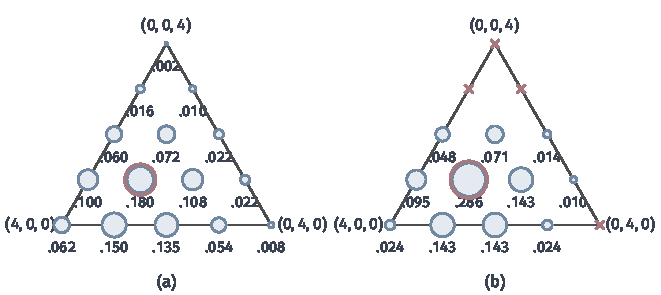
\includegraphics[width=112mm]{figures/07-probability/01-elementary-probability/matplotlib/mvd-count-lattice/figure.pdf}
  \caption{总和为$4$的三类计数的联合分布，每个格点代表一个计数向量$(k_1,k_2,k_3)$，圆的面积与概率成正比，下方数字是概率。(a)多项分布$\operatorname{Mult}(4,(0.5,0.3,0.2))$。(b)从$5$红、$3$绿、$2$黄共$10$个球中不放回摸$4$个的多元超几何分布；红叉是不可能出现的计数。红圈标出$(2,1,1)$。}
  \label{fig:mvd-count-lattice}
\end{BookInlineFigure}

\paragraph{合并类别与边缘分布}
只关心第$1$类时，可以把其余类别合成“非第$1$类”。每次试验仍然相互独立，落入第$1$类的概率仍是$p_1$，所以$N_1$就是$n$次独立试验中的成功次数：
\[
 N_i\sim\operatorname{Bin}(n,p_i),\qquad i=1,\ldots,d .
\]
更一般地，把若干类别合并成一类，合并后的计数仍服从多项分布，参数是对应概率之和。例如甜品店中把口味$1,2$合并，
\[
 (N_1+N_2,\ N_3)\sim\operatorname{Mult}\bigl(4,(0.8,0.2)\bigr) .
\]
这种做法不需要对式~\eqref{eq:mvd-multinomial-pmf}求和，它直接回到试验机制：合并类别只是把记录方式变粗，独立重复的结构没有改变。

\paragraph{示性变量与协方差}
计数的均值和协方差最好通过逐次记录来算。对第$t$次试验和第$i$类，令示性变量
\[
 I_{t,i}=\mathbf{1}_{\{\text{第}t\text{次落入第}i\text{类}\}},\qquad N_i=\sum_{t=1}^{n}I_{t,i} .
\]
把$I_{t,i}$排成$n$行$d$列的表，图~\ref{fig:mvd-indicator-table}画出了序列$1,3,1,2$对应的表，列和就是计数。

\begin{BookInlineFigure}
  \centering
  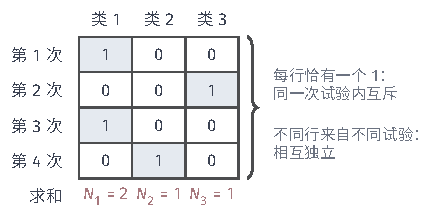
\includegraphics[width=73mm]{figures/07-probability/01-elementary-probability/tikz/mvd-indicator-table/figure.pdf}
  \caption{四次试验、三个类别的示性变量表，对应结果序列$1,3,1,2$。每一行恰有一个$1$（浅蓝），各列之和给出计数$\bm{N}=(2,1,1)$。同一行内的示性变量互斥，不同行来自相互独立的试验。}
  \label{fig:mvd-indicator-table}
\end{BookInlineFigure}

表中有两种关系。同一行的$d$个示性变量互斥：一次试验只能落入一个类别，所以$i\neq j$时$I_{t,i}I_{t,j}=0$。不同行来自不同试验，相互独立。前者产生负的协方差，后者不产生任何交叉项。

\begin{theorem}[多项计数的均值与协方差]
\label{thm:mvd-multinomial-moments}
设$\bm{N}\sim\operatorname{Mult}(n,\bm{p})$，则$\mathbb{E}[\bm{N}]=n\bm{p}$，并且
\begin{equation}
 \operatorname{Cov}(N_i,N_j)=
 \begin{cases}
  np_i(1-p_i), & i=j,\\
  -np_ip_j, & i\neq j .
 \end{cases}
 \label{eq:mvd-multinomial-cov}
\end{equation}
用矩阵写，即
\begin{equation}
 \operatorname{Cov}(\bm{N})=n\bigl(\operatorname{diag}(\bm{p})-\bm{p}\bm{p}^{\top}\bigr) .
 \label{eq:mvd-multinomial-cov-matrix}
\end{equation}
\end{theorem}

\begin{proof}
每个$I_{t,i}$只取$0,1$，取$1$的概率是$p_i$，所以$\mathbb{E}[I_{t,i}]=p_i$，对$t$求和得$\mathbb{E}[N_i]=np_i$。

协方差对两个变量都是线性的，展开两个和式，
\[
 \operatorname{Cov}(N_i,N_j)=\sum_{t=1}^{n}\sum_{s=1}^{n}\operatorname{Cov}(I_{t,i},I_{s,j}) .
\]
$t\neq s$时两个示性变量来自不同试验，相互独立，协方差为$0$。只剩$t=s$的$n$项。

同一次试验中，$i=j$时$I_{t,i}^{2}=I_{t,i}$；$i\neq j$时$I_{t,i}I_{t,j}=0$。于是
\[
 \operatorname{Cov}(I_{t,i},I_{t,j})=\mathbb{E}[I_{t,i}I_{t,j}]-p_ip_j=
 \begin{cases}
  p_i-p_i^{2}, & i=j,\\
  -p_ip_j, & i\neq j .
 \end{cases}
\]
乘以$n$即得式~\eqref{eq:mvd-multinomial-cov}。
\end{proof}

对甜品店，$n=4$，$\bm{p}=(0.5,0.3,0.2)^{\top}$，代入式~\eqref{eq:mvd-multinomial-cov}，协方差矩阵是
\[
 \begin{bmatrix}
  1 & -0.6 & -0.4\\
  -0.6 & 0.84 & -0.24\\
  -0.4 & -0.24 & 0.64
 \end{bmatrix} .
\]
对角元是三个二项分布的方差，非对角元全为负：一位顾客选了口味$1$，就不能再选口味$2$。

这个矩阵每一行的和都是$0$。一般地，第$i$行之和为$np_i-np_i\sum_jp_j=0$，即协方差矩阵乘以全一向量$\bm{1}$得零向量。这与总和约束一致：
\[
 \operatorname{Var}(N_1+\cdots+N_d)=\bm{1}^{\top}\operatorname{Cov}(\bm{N})\bm{1}=0 ,
\]
常数$n$没有波动。所以多项分布的协方差矩阵总是奇异的。

当各$p_i>0$时，$\bm{1}$的倍数是零空间中仅有的方向。若式~\eqref{eq:mvd-multinomial-cov-matrix}的矩阵把$\bm{v}$映成零向量，第$i$个分量给出$p_iv_i=p_i(\bm{p}^{\top}\bm{v})$，除以$p_i$得$v_i=\bm{p}^{\top}\bm{v}$，各分量相等。因此协方差矩阵的秩是$d-1$，与格点三角形的维数相同。

负协方差说明分量相关，因而不独立。也可以直接看一个事件：$\mathbb{P}(N_1=4)=0.0625$，$\mathbb{P}(N_2=4)=0.0081$，两者都为正，可是$N_1=4$与$N_2=4$不能同时发生，联合概率是$0$，不等于乘积。把各类计数当成独立的二项变量，会给不可能的组合分配正概率。

\subsection{多元超几何分布}
\label{sec:mvd-multivariate-hypergeometric}

\paragraph{联合质量函数}
现在换成摸球。总体有$M$个对象，第$i$类有$K_i$个，$K_1+\cdots+K_d=M$；从中一次不放回地取出$n$个，$1\leq n\leq M$，每个$n$元子集被取到的机会相同。仍用$N_i$记取出的第$i$类个数。

所有可能的子集共有$\binom{M}{n}$个。取出的结果恰好含$k_i$个第$i$类对象，相当于在每一类里各自挑$k_i$个，挑法数相乘，于是得到下面的定义。

\begin{definition}[多元超几何分布]
\label{def:mvd-multivariate-hypergeometric}
设各类数目$K_i$为非负整数，$M=\sum_iK_i$，$1\leq n\leq M$。若
\begin{equation}
 \mathbb{P}(\bm{N}=\bm{k})=\frac{\binom{K_1}{k_1}\binom{K_2}{k_2}\cdots\binom{K_d}{k_d}}{\binom{M}{n}},
 \label{eq:mvd-mhyper-pmf}
\end{equation}
其中$\bm{k}$取遍满足$0\leq k_i\leq K_i$、$k_1+\cdots+k_d=n$的整数向量，则称$\bm{N}$服从\term{多元超几何分布}（multivariate hypergeometric distribution）。
\end{definition}

与多项分布相比，取值多了上限$k_i\leq K_i$：盒子里只有$2$个黄球，就不可能摸出$3$个。在摸球例子中，$M=10$，$\bm{K}=(5,3,2)$，$n=4$，$\binom{10}{4}=210$。计数$(2,1,1)$的概率是
\[
 \frac{\binom{5}{2}\binom{3}{1}\binom{2}{1}}{210}=\frac{10\times3\times2}{210}=\frac{2}{7}\approx0.286 ,
\]
比多项分布的$0.18$大。图~\ref{fig:mvd-count-lattice}(b)画出全部格点：黄球数为$3$或$4$、绿球数为$4$的格点概率为$0$，用红叉标出；剩下的质量更集中在中间。

\paragraph{逐次抽取的对称性}
求均值和协方差时，把“一次取出$n$个”想成依次取出$n$个、每次在剩下的对象中等可能地取一个。这样得到的有序结果共有$M(M-1)\cdots(M-n+1)$种，每种机会相同，忽略顺序就回到等可能的子集。仍记$I_{t,i}$为第$t$次取到第$i$类的示性变量，$N_i=\sum_tI_{t,i}$。

关键是一个对称性：第$t$次取到的对象在全体$M$个对象上等可能。数一数就知道：指定第$t$次取对象$o$，其余$n-1$个位置从剩下的$M-1$个对象中依次挑选，有序结果的条数与$o$是哪一个无关。同理，对$t\neq s$，第$t$次与第$s$次取到的有序对在所有$M(M-1)$个“不同对象的有序对”上等可能。

记$q_i=K_i/M$为第$i$类的比例。由第一条对称性，$\mathbb{P}(I_{t,i}=1)=q_i$。由第二条，$t\neq s$时，
\[
 \mathbb{P}(I_{t,i}=1,\ I_{s,j}=1)=
 \begin{cases}
  \dfrac{K_i(K_i-1)}{M(M-1)}, & i=j,\\
  \dfrac{K_iK_j}{M(M-1)}, & i\neq j .
 \end{cases}
\]
这里需要$M\geq2$。不同次的抽取不再独立：先取走一个第$i$类对象，第$i$类在剩余对象中的比例就变小了。

\begin{theorem}[多元超几何计数的均值与协方差]
\label{thm:mvd-mhyper-moments}
设$\bm{N}$服从定义~\ref{def:mvd-multivariate-hypergeometric}的分布，$M\geq2$，$\bm{q}=\bm{K}/M$。则$\mathbb{E}[\bm{N}]=n\bm{q}$，并且
\begin{equation}
 \operatorname{Cov}(\bm{N})=n\,\frac{M-n}{M-1}\bigl(\operatorname{diag}(\bm{q})-\bm{q}\bm{q}^{\top}\bigr) .
 \label{eq:mvd-mhyper-cov}
\end{equation}
\end{theorem}

\begin{proof}
均值由$\mathbb{E}[I_{t,i}]=q_i$对$t$求和得到。协方差仍按双重和展开，分成$t=s$的$n$项和$t\neq s$的$n(n-1)$项。同一次抽取内的情形与多项分布完全一样，贡献$n(\delta_{i,j}q_i-q_iq_j)$，其中$\delta_{i,j}$在$i=j$时为$1$、否则为$0$。

先算$i\neq j$。由上面的联合概率，$t\neq s$的每一项是
\[
 \frac{K_iK_j}{M(M-1)}-q_iq_j=q_iq_j\Bigl(\frac{M}{M-1}-1\Bigr)=\frac{q_iq_j}{M-1} .
\]
两部分相加，
\[
 \operatorname{Cov}(N_i,N_j)=-nq_iq_j+\frac{n(n-1)q_iq_j}{M-1}=-nq_iq_j\,\frac{M-n}{M-1} .
\]

再算$i=j$。$t\neq s$的每一项是
\[
 \frac{K_i(K_i-1)}{M(M-1)}-q_i^{2}=q_i\,\frac{(K_i-1)M-K_i(M-1)}{M(M-1)}=-\frac{q_i(1-q_i)}{M-1} .
\]
与$t=s$的贡献$nq_i(1-q_i)$相加，
\[
 \operatorname{Var}(N_i)=nq_i(1-q_i)\Bigl(1-\frac{n-1}{M-1}\Bigr)=nq_i(1-q_i)\,\frac{M-n}{M-1} .
\]
两种情形合起来就是式~\eqref{eq:mvd-mhyper-cov}。
\end{proof}

\paragraph{与多项分布的比较}
取多项分布的$\bm{p}$等于总体比例$\bm{q}$，两种抽样的均值完全相同，协方差的形状也相同，只差一个因子$(M-n)/(M-1)$。$n\geq2$时这个因子小于$1$：不放回抽样的计数波动更小。直观上，摸出一个红球后剩下的红球变少，下一次摸到红球的机会随之下降，这种负反馈把计数往总体比例上拉。

摸球例子中，因子是$(10-4)/(10-1)=2/3$。红球数的方差从多项分布的$1$降到$2/3$，红、绿两类的协方差从$-0.6$变成$-0.4$。极端情形$n=M$时因子为$0$：整盒取出，计数恒等于$\bm{K}$，没有任何随机性。$n=1$时因子为$1$，一次抽取放回与否没有区别。

总和约束对两种模型同样起作用。$\operatorname{diag}(\bm{q})-\bm{q}\bm{q}^{\top}$的行和为$0$，所以式~\eqref{eq:mvd-mhyper-cov}同样是奇异矩阵，各类计数两两负相关。

\paragraph{何时可以用多项分布近似}
直观上，总体很大而只取少数几个时，取走的对象几乎不改变剩余组成，不放回与放回应当相差无几。下面的结论把这一点说准确。

\begin{theorem}[大总体下的多项近似]
\label{thm:mvd-mhyper-limit}
固定$n$、$d$和满足$\sum_ik_i=n$的非负整数向量$\bm{k}$。让总体规模$M\to\infty$，各类数目$K_i=K_i(M)$满足$K_i/M\to q_i$，则式~\eqref{eq:mvd-mhyper-pmf}的概率趋于$\operatorname{Mult}(n,\bm{q})$在$\bm{k}$处的概率。
\end{theorem}

\begin{proof}
把二项式系数写成阶乘之比，式~\eqref{eq:mvd-mhyper-pmf}改写为
\[
 \frac{n!}{k_1!\cdots k_d!}\cdot
 \frac{\prod_{i=1}^{d}K_i(K_i-1)\cdots(K_i-k_i+1)}{M(M-1)\cdots(M-n+1)} .
\]
第一个因子就是多项式系数。第二个因子的分子共有$\sum_ik_i=n$个因子，分母也是$n$个因子。

把分子分母的因子一一配对，每一对形如$(K_i-a)/(M-b)$，其中$a<k_i$、$b<n$都是固定整数。$M\to\infty$时，
\[
 \frac{K_i-a}{M-b}=\frac{K_i/M-a/M}{1-b/M}\to q_i .
\]
第$i$类恰好贡献$k_i$对，所以第二个因子趋于$\prod_iq_i^{k_i}$，与第一个因子相乘即为式~\eqref{eq:mvd-multinomial-pmf}。
\end{proof}

定理只说极限，实际使用时还要看差多少。协方差的因子$(M-n)/(M-1)$与$1-n/M$相差不到$1/(M-1)$，所以抽样比例$n/M$是主要的判断依据。图~\ref{fig:mvd-hypergeom-approx}保持红球比例$0.5$、$n=4$：$M=10$时红球数的分布明显比$\operatorname{Bin}(4,0.5)$集中，$M=40$时已经相当接近。右图说明方差因子几乎落在直线$1-n/M$上。

\begin{BookInlineFigure}
  \centering
  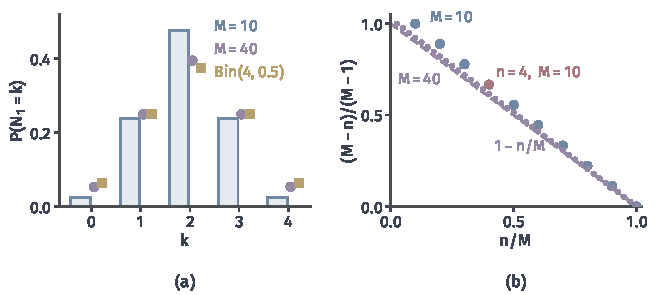
\includegraphics[width=112mm]{figures/07-probability/01-elementary-probability/matplotlib/mvd-hypergeom-approx/figure.pdf}
  \caption{不放回与放回抽样的比较，第$1$类比例$0.5$，抽取$n=4$个。(a)第$1$类计数$N_1$的质量函数：总体$M=10$（蓝色柱）、$M=40$（紫点）与$\operatorname{Bin}(4,0.5)$（黄色方块）。(b)方差因子$(M-n)/(M-1)$随抽样比例$n/M$的变化，蓝点为$M=10$，紫点为$M=40$，紫色虚线为$1-n/M$；红点是本节例子$n=4$、$M=10$。}
  \label{fig:mvd-hypergeom-approx}
\end{BookInlineFigure}

具体数值是：$M=10$时$\mathbb{P}(N_1=2)=100/210\approx0.476$，$M=40$时约为$0.395$，二项分布为$6/16=0.375$。抽样比例从$0.4$降到$0.1$，差距从$0.10$缩小到$0.02$。抽样比例不小时，应当保留有限总体的结构，否则会高估计数的波动，还会给超出$K_i$的计数分配概率。
